\documentclass{llncs}
\pagestyle{plain}

\usepackage[T1]{fontenc}
\usepackage{amsfonts}
\usepackage{graphicx}
\usepackage[ruled]{algorithm2e} % For algorithms
\usepackage{stix}

\newcommand{\text}[1]{\textrm{#1}}
\bibliographystyle{splncs04}

\title{Population-Based Algorithms \\
 Built on Weighted Automata}
%
\titlerunning{Automata as compressed populations}
%% \titlerunning{}

\author{Gijs Schr\"oder\inst{1}\orcidID{0000-0001-6803-3237} \and Inge Wortel\inst{1}\orcidID{0000-0003-3362-5229}  \and Johannes~Textor\inst{1}\orcidID{0000-0002-0459-9458}}

\institute{Institute for Computing and Information Sciences, \\ Radboud University, 
Nijmegen, The Netherlands \\ \email{\{gijs.schroeder,inge.wortel,johannes.textor\}@ru.nl} }

\authorrunning{G. Schr\"oder et al.}
%\and \email{inge.wortel@ru.nl} \and \email{johannes.textor@ru.nl}}

\begin{document}

\maketitle

\begin{abstract}

  Many algorithms in natural computing and computational biology are
population-based: genetic algorithms evolve candidate solutions for
optimization problems; artificial immune systems and learning classifier
systems maintain populations of rules. Using such algorithms at very large
population sizes (e.g., millions or billions) is computationally
expensive.  Here, we develop a methodology for implementing population-based
models using  weighted finite state machines (WFSMs) with exact rational
weights.  For populations that can be represented as weighted sets of strings,
WFSMs can reduce memory use and runtime of population-based algorithms by
orders of magnitude.  We demonstrate the generality of our approach by
constructing an immune-inspired anomaly detector for string data and an
evolutionary algorithm that solves Boolean satisfiability problems.  The WFSM
approach allows repurposing of advanced algorithms developed for natural
language processing, and should be applicable to other population-based
algorithms such as learning classifier systems.

  \keywords{Simulation tools \and Regular languages \and Weighted automata}
\end{abstract}


\section{Introduction}

Many algorithms in computer science perform a search, optimization, or learning procedure by maintaining and evolving a set of points in some kind of search space. Such \emph{population-based} algorithms \cite{Blum_2003} encompass nature-inspired metaheuristics like evolutionary algorithms (EAs) \cite{Jansen2013}, ant colony optimization \cite{Blum2005}, particle swarm optimization \cite{Gad2022}, and artificial immune systems \cite{Timmis2004}, but are not only used in natural computing: various more classical algorithms such as the approximate Bayesian computation method for parameter inference \cite{Sisson2007} %% , Markov Chain Monte Carlo methods,
or simulated annealing can also be viewed as population-based.

This paper focuses on populations that can be represented as sets of strings with associated weights, such as, for instance, EAs with real-valued fitness functions. We ask a simple question: how can we efficiently implement such algorithms when the population sizes are very large -- say, in the millions? While small populations are fine in some cases (even a simple 1+1-EA  successfully solves many problems), large populations can be required to tackle complex, high-dimensional problems in many areas, such as anomaly detection by immune-inspired classifier systems \cite{Stibor2005}. 

An obvious approach to deal with large populations is parallelization, which is typically straightforward and achieves linear runtime improvement. Here we use a different approach that has been much less explored: \emph{population compression}. While being more difficult to implement, it can, in some cases, achieve superlinear or even exponential gains \cite{Liskiewicz2010}. To our knowledge, the idea of population compression first appeared in the field of artificial immune systems (AIS) \cite{Elberfeld_2009}, where it was used to build the first polynomial-time immune-inspired classification algorithms, a feat that had previously been considered unachievable as it was thought to be an NP-hard problem \cite{Timmis2008}. In these algorithms, population compression is achieved by representing the ``detectors'' comprising the population -- which are simply strings -- as a finite state machine (FSM). For large string sets with regular structure, FSMs can be exponentially smaller than an explicit list of the population. Recently, the FSM approach was used to build a computational model of T~cell populations in the human immune system that contained tens of millions of ``detectors'' and processed the entire human proteome as input \cite{Wortel2020t}. 

It is not straightforward to use FSM-based population compression methods in other population-based algorithms as existing methods are still relatively limited. Crucially, FSMs represent populations as sets without multiplicity. This means that all individuals in the population are qualitatively equal, limiting the types of operations that can be performed on them. For instance, in an EA, we may wish to sample new candidates for reproduction in a fitness-dependent manner; this kind of operation is not supported by existing FSM-based approaches.

In this paper, we will extend population compression methods developed for AIS in a manner
that makes them useable for more general population-based algorithms. Specifically, we 
offer the following contributions: 

\begin{enumerate}
\item We present a population compression approach based on \emph{weighted} FSMs (WFSMs) with rational
edge weights (Section~\ref{sectionfsms}). This approach allows us to augment the compressed population with important information such as multiplicity or fitness. 
\item We use WFSMs to implement a weighted version of positive selection, a key AIS classification algorithm, and show that the addition of weights can lead to higher accuracy and robustness compared to the unweighted baseline (Section~\ref{sectionempirical}).
\item We use WFSMs to implement an EA that solves the Boolean satisfiability problem (Section~\ref{sectionwaga}).
%this approach to define weighted versions of positive and negative selection, two of the most important AIS algorithms, and show that the addition of weights can lead to higher accuracy and robustness compared to unweighted baselines (Section~\ref{sectionempirical});

%\item Show how weighted positive and negative selection can be implemented efficiently by using compressed repertoire representations based on weighted FSMs (Section~\ref{sectionfsms});
%\item Illustrate the potential benefit of using weights by comparing the performance of weighted versus unweighted repertoire models on simple string-based anomaly detection problems (Section~\ref{sectionempirical}).
\end{enumerate}


We have implemented our WFSM-based algorithms in C++, making heavy use of the library OpenFST \cite{openfst}. An implementation is available for download at Zenodo \cite{CodeForPaper}.

\section{Background}

\label{sectionbackground}

We consider strings $x$ over some finite alphabet $\Sigma$.
%Lowercase Latin letters denote strings.
E.g., $x=0010 \in \{0,1\}^4$ is a string consisting of 4 binary characters and $x_3=1$ is its third character.
The symbol $\ell$ is always the length of some string.
We write $|S|$ to denote the cardinality of a set $S$.

A \emph{population} is a set of strings -- e.g., the genotypes in an EA.
A \emph{weighted population} consists of a population $S$ and a mapping $w : S \mapsto \mathbb{Q}$ that associates a rational number to each string in $S$ (see~Section~\ref{sectionwhyrationals} for why we choose rationals).
For clearer distinction, a population $S$ is also called an \emph{unweighted population}.
Unweighted populations are interchangeable with weighted populations with unit weights.

The weights can have different interpretations:
positive integer weights could be used to simply store multiplicity of individuals in the population,
whereas fractional weights could represent each individual's importance or fitness.
Weights in the interval $(0,1]$ could represent probabilities of being present in the set.%%  that each element is actually present in the set.

In the following, let $(S, w_S)$, $(T, w_T)$, and $(U, w_U)$ each be weighted populations.
For simplicity, let $w_A(x)=0$ if $x \notin A$ and let $f = g \star h$ denote $f(x) = g(x) \star h(x)$, where $\star$ is any operation.
In a slight abuse of notation, we define three binary operations for two populations $(S, w_S)$ (abbreviated as $S$) and
$(T, w_T)$ (abbreviated as $T$):

$S \uplus T = U$ is the \emph{sum} of $S$ and $T$, where $U = S \cup T$ and $w_U = w_S + w_T$.

$S \capdot T = U$ is the \emph{product} of $S$ and $T$, where $U = S \cap T$ and $w_U = w_S \times w_T$.

$S \setminus T = U$ is the \emph{set difference} of $S$ and $T$, where $U = S \setminus T$ and $w_U = w_S$.

%% This notation is chosen to be distinct from set operations where possible.

%We define these three operations in particular,
%because they correspond closely to known constructions on weighted finite state machines ().

%% We include a definition of WFSMs for completeness,
%% but note that it can be safely skipped on a first reading.

A \emph{weighted finite state machine} (WFSM) over an alphabet $\Sigma$ and a semiring $\mathbb{K}$ is a 6-tuple $M = (Q, E, \sigma, k, q_0, F)$,
where $(Q,E)$ is a directed graph of states as vertices,
with \emph{initial} state $q_0 \in Q$ and \emph{final} states $F \subseteq Q$.
Edges $q_i \to q_j$ are labeled by characters $\sigma : E \mapsto \Sigma$ and \emph{weights} $k : E \mapsto \mathbb{K}$.
An example WFSM is shown in Figure~\ref{fig:fsa-ex}B.

This $M$ defines a language $\mathcal{L}(M) \subseteq \Sigma^*$ and an associated function $w_M : \Sigma^* \mapsto \mathbb{K}$ by its graph structure and edge labels.
For $q_\ell \in F$,
an \emph{accepting path} $\pi = q_0 \to \ldots \to q_\ell$ is
\emph{labeled} $x = \sigma(q_0 \to q_1) \ldots \sigma(q_{\ell-1} \to q_\ell)$
and has \emph{weight} $k(\pi)=\prod_{j=0}^{\ell-1} k( q_j \to q_{j+1} )$,
where $\prod$ uses the product operator in $\mathbb{K}$.
The weight $w_M(x)$ of a string $x$ is the sum of all weights of accepting paths labeled with $x$, or zero in absence of such paths.

A WFSM is \emph{deterministic} if no two edges from the same source
state are labeled with the same character.
A deterministic WFSM is called \emph{minimal} if it has the least
number of states out of all deterministic WFSMs accepting the same
language and weights.
To \emph{minimize} a deterministic WFSM is to find a corresponding minimal WFSM. %% $M$ is to find a minimal WFSM accepting $\mathcal{L(M)}$ with weights $w_M$.

Ordinary FSMs without weight can be recovered from WFSMs by
substituting for $\mathbb{K}$ the two-element Boolean algebra.
If we let $\mathbb{K}=\mathbb{Q}$ instead,
then any WFSM $M$ defines a set of strings $\mathcal{L}(M)$ and an
associated $w_M$ that together constitute a weighted population.
The three operations defined above can then be implemented with
weighted variants of union, intersection, and difference constructions.
Restricting ourselves to deterministic WFSMs,
we can compress these WFSMs by minimization.

%% Define a \emph{path} to be a sequence of states, $q_1 \ldots q_\ell$,
%% such that $q_i \to q_{i+1} \in E$ for each $i$ in $1 \ldots \ell-1$.
%% An \emph{accepting path} has both both $q_1 \in I$ and $q_\ell \in F$.
%% For such paths, $x = a(q_1 \to q_2) \ldots a(q_{\ell-1} \to q_\ell)$ is in $L$.
%% Define $P(x)$ to be the set of accepting paths that are labeled by the string $x$.
%% Then the weight of $x$ is $w(x) = \bigoplus_{\pi \in P(x)} \bigotimes_{i=1}^\ell b(q_i \to q_{i+1})$,
%% with $\oplus$ and $\otimes$ being addition and multiplication in $\mathbb{K}$.


%% A WFSM $M=(Q,E,c,w,q_s, Q_F)$ over an alphabet $\Sigma$ and a semiring $\mathbb{K}$ consists of a 
%% directed graph $G=(Q,E)$ linking states $q \in Q$ where the state $q_s \in Q$ is called the 
%% \emph{initial (starting) state} and the states $Q_F \subseteq Q$ are called the 
%% \emph{accepting (final) states}. 
%% The edges \emph{(transitions)} $q_i \to q_j \in E$  are labeled by 
%% characters $c : E \mapsto \Sigma$ and weights $w : E \mapsto \mathbb{K}$. 


%% Throughout this paper, the term \emph{population} refers to a set of strings -- e.g., the genotypes in an evolutionary algorithm.
    %% A \emph{weighted population} consists of a population $S$ and a mapping $w : S \to \mathbb{R}$, though we implement this $w$ with a rational representation for reasons explained below.
    %% where $\mathcal{W}$ is a set of weights; typical examples are $\mathcal{W} = \mathbb{R}$ or $\mathcal{W} = \mathbb{Z}$, although throughout  this paper, we will use $\mathcal{W} = \mathbb{Q}$ for reasons explained below.

\subsection{Compressing unweighted populations}

\label{sectionunweightedrep}

We now briefly review the existing approach from the AIS field where finite state machines
(FSMs) are used as compressed representations of populations.
This review %% is important to 
delineates what this approach %% the existing approach
can already accomplish and where it currently falls short.

The AIS algorithms we will consider are classifiers 
%that can alternatively be thought of as very 
%simple learning classifier systems. They 
that are based on populations of so-called 
%
%We use the term \emph{repertoire model} in this paper to denote a type of AIS that is 
%loosely based on T~cell and B~cell receptor repertoires in the real immune system. 
\emph{detectors},
%% (also called patterns)
where each detector is a string that represents
a small part of a set $\mathcal{U}$ (universe) of objects to classify. By extension, detector populations can therefore 
represent  (``cover'') subsets of $\mathcal{U}$. Although this framework is general and allows 
$\mathcal{U}$ to be any set, in this paper we focus on strings over some alphabet 
$\Sigma$, where each string consists of $\ell$ characters ($\mathcal{U}=\Sigma^\ell$).

% since the generalization of our framework to variable-length 
%strings is reasonably straightforward. 

In addition to the \emph{universe}: $\mathcal{U}$ that represents the objects to be classified, we define a set of \emph{detectors} $\mathcal{D}$; possibly $\mathcal{U}=\mathcal{D}$. A \emph{matching function} $m : \mathcal{D} \mapsto 2^\mathcal{U}$, where $2^\mathcal{U}$ denotes the powerset of $\mathcal{U}$, associates every detector with the elements it recognizes. We define the inverse matching function $m^{-1} : \mathcal{U} \mapsto 2^\mathcal{D}$ as $m^{-1}(x) = \{ d \in \mathcal{D} \mid x \in m(d) \} $. In this setting, a population is simply a subset of $\mathcal{D}$. 

\begin{definition}[Matching rules]
Given an alphabet $\Sigma$ and a string length $\ell$, we define the following matching rules:
\begin{enumerate}
%% \item \emph{Wildcard pattern matching:} considers a wildcard symbol $\# \notin \Sigma$ 
%% and sets $\mathcal{U}=\Sigma^\ell, \mathcal{D}=\Sigma \cup \{\#\}^\ell$. 
%% Then $m(x) = \{ y \in \mathcal{U} : \forall i \in \{1,\ldots,n\} : x_i \in \{ y_i, \# \} \}$. 
 \item \emph{r-Contiguous matching:}  $\mathcal{U}=\mathcal{D}=\Sigma^\ell$, $m_r(x)=\{y \in \mathcal{U} : \exists i \in \{1,\ldots,\ell-r+1\} : \forall j \in \{i,\ldots,i+r-1\} : x_j = y_j \}$; in words, $x$ and $y$ have at least $r$ identical
consecutive characters. 
 The parameter $r$, called \emph{matching radius}, controls the number of strings each 
 detector matches: increasing $r$ means matching fewer strings. This pattern matching 
 rule is common in AIS.
\item \emph{r-Hamming matching:} $m_r(x)=\{y \in \mathcal{U} : |\{ i : x_i \neq y_i \}| \leq r \}$;
in words, $x$ and $y$ have at most $r$ non-identical characters.
Here, increasing the matching radius $r$ means matching more strings.
\end{enumerate}
\label{definitionmatchingrules} % 2 references
\end{definition}

Using any such matching rule, we can build classification algorithms based on detector 
populations. 
Inspired by the way that T~cells are generated and selected in real immune systems,
there are two main population-based classification algorithms that were studied in the AIS field. 
Both are so-called \emph{one-class} classification algorithms that take an input 
sequence $S \in \mathcal{U}^*$ (also called \emph{self}) to construct a detector population $P$, 
which is then used to determine whether the elements of a second input sequence $T \in \mathcal{U}^*$ 
belong to the same class as the elements of $S$:

\begin{definition}[Positive and negative selection]
For an input sequence  $S=(s_1,\ldots,s_n)$, $S \in \mathcal{U}^n$,
a detector type $\mathcal{D}$ and a matching function $m$,  we call a 
detector population $P \subseteq \mathcal{D}$
\begin{enumerate}
\item \emph{positively selected} if $P \subseteq \bigcup_i m^{-1}(s_i)$ is a set of detectors 
that match at least one input string.
\item \emph{negatively selected} if $P \subseteq \mathcal{D} \setminus \bigcup_i m^{-1}(s_i)$ 
is a set of detectors that do not match any input string. 
\end{enumerate}

A negatively (positively) selected population $P$ is \emph{maximal} if there is no strict superset of $P$ that is also negatively (positively) selected with respect to the same input $S$. Given a population $P$ and an element $t \in \mathcal{U}$, we define the \emph{scoring function} $P(y) =  |P \cap m^{-1}(y)|$ as the number of detectors in $P$ that match $y$. 
\label{definitionposnegsel} % 2 references
\end{definition}

For a positively selected population, the scoring function can be understood as a \emph{normalcy score} (a high value $P(y)$ means that $y$ is ``similar to'' $S$) whereas for negative selection, the interpretation is the opposite (\emph{anomaly score}). The scores output by a positively or negatively selected population can be used for threshold-based classification. Note that we did not define which specific detectors are used, only which detectors \emph{could} be in the population. A simple method is generating detectors by rejection sampling. However, depending on the input, rejection rates can be high \cite{Dhaeseleer1996,Dhaeseleer1996b}, while at the same time huge populations can be required to achieve acceptable classification results %% can be exponential in the input
\cite{Stibor2005}. 

These issues motivated the development of population compression 
techniques \cite{Elberfeld_2009,Elberfeld2011}.
The basic idea is that FSMs can compactly represent large sets of strings with 
shared structure (Figure~\ref{fig:fsa-ex}A). This representation has several advantages.
For any given population $P$, the smallest FSM that represents $P$ can be computed in polynomial time in the 
size of $P$. The operations that are required to implement positively and negatively selected populations,
such as union, intersection, set difference, and computation of cardinality, can all be efficiently performed directly 
on the FSM representation.  Since FSMs are generic data structures, this approach benefits 
from a large body of work done to develop efficient FSM algorithms and high-quality, mature software implementations 
such as the OpenFST framework \cite{openfst}. 
The FSM-based approach can improve runtime by orders of 
magnitude \cite{Textor2012,Textor2014}. The key requirement is that we need to be able to efficiently generate
an FSM that represents the population $m^{-1}(s_i)$ (Definition~\ref{definitionposnegsel}); whether this is possible
depends on the matching rule that is used.

\begin{figure}[t]
  \begin{tabular}{p{0.5em}@{}cp{0.5em}@{}c}
    \raisebox{-\height}{A} &
    \raisebox{-\height}{\includegraphics{figures/drawing.eps}}
    \raisebox{-\height}{B} &
    \raisebox{-\height}{\includegraphics{figures/wfsm-table.eps}}
  \end{tabular}
  \caption{
    FSMs as compact representations of sets of strings.
    (A)
    FSMs encoding the string set $\{a,b\}^\ell$ for $\ell \in \{1,2,3\}$. Although the string sets
    grow exponentially in size as a function of $\ell$, FSM size is linear in $\ell$.
    (B)
    A weighted FSM, along with a table showing the strings it contains and the associated weights for
    these strings. Path transitions are labeled (character/weight). 
    Each unique path represents a string (the concatenation of every such character along 
    the path) with its associated weight (the product of every weight along the path).
  }
  \label{fig:fsa-ex}
\end{figure}

If we are able to employ the FSM approach, we no longer need to generate populations by random sampling and 
can instead just directly use maximal detector populations \cite{Textor2012,Textor2014}. 
Interestingly, although positive and negative selection using randomly generated detectors can give different 
results, for many matching rules this is not the case when maximal detector sets are used.

%\newtheorem{remark}{Remark}

\begin{remark}
For the matching rules in Definition~\ref{definitionmatchingrules}, 
positive and negative selection with maximal detector sets are equivalent classifiers.
\label{remarkbotharethesame}
\end{remark} 

\begin{proof}
If $P^+$ and $P^-$ are the maximal positively and negatively selected detector populations w.r.t. an input $S$, 
then we have $P^+ \cup P^- = \mathcal{D}$ and therefore 
%$(D^+\cap m^{-1}(t)) \cup (D^-\cap m^{-1}(t)) =  m^{-1}(t)$. Therefore 
$|P^+ \cap m^{-1}(y)|
+ |P^- \cap m^{-1}(y)|=|m^{-1}(y)|$. Since $|m^{-1}(y)|$ is the same value for all $y \in \mathcal{U}$ 
for the matching rules in Definition~\ref{definitionmatchingrules}, the scoring function of negative 
selection is a constant minus the scoring function of positive selection, and vice versa.
\end{proof}

Beyond positive and negative selection, further operations that could be performed with FSM-compressed classifier populations include sampling from $P$ or incrementally modifying $P$ \cite{Textor2014}. However, some important limitations remain. Crucially for classification tasks, negative and positive selection do not take into account possible multiplicity of strings in the input sequences. In many real-world cases, it is important to distinguish, say, an input element that occurs once in the training data from another that occurs thousands of times. Moreover, AIS classifiers process the entire input data only once. Many other population-based algorithms modify the populations in more complex ways that require, for instance, weighted sampling from the population or pruning of low-weight elements from the population. Such operations are not supported by FSM-compressed populations.

\section{Weighted Population Compression}
\label{sectionfsms}\label{sectionwhyrationals}

We extend the FSM-based population compression approach explained in
the previous section to \emph{weighted} populations as defined in
Section~\ref{sectionbackground}.
We aim to compress the weighted populations with WFSMs and to
implement the three weighted population operators using WFSM
algorithms.

These WFSMs are preferably as small as possible.
However, using conventional floats for edge weights instead of
rationals causes WFSMs to explode in size with the number of
operations performed on them.
This is no minor issue;
for the algorithms described in the next section,
this size explosion prevented us from doing any testing on
real data. We will demonstrate the issue and its solution
using a simple task.

\begin{figure}[t]
  \centering
  \begin{tabular}{p{0.5em}@{}cp{0.5em}@{}c}
    \raisebox{-\height}{A} &
    \raisebox{-\height}{\includegraphics{figures/diagram.eps}} &
    \raisebox{-\height}{B} &
    \raisebox{-\height}{\includegraphics{figures/states3.pdf}}
  \end{tabular}
  \caption{
    Exact arithmetic helps keeping WFSMs small.
    (A) Weighted union between two WFSMs, using exact and inexact arithmetic.
    With exact arithmetic the path weight for $bb$ is $\frac{1}{7} \times 7=1$,
    which can be merged with $ab$'s path weight of $1$ to obtain a small WFSM (bottom left, blue).
    However, with inexact arithmetic this weight becomes $0.14 \times 7=0.98$,
    which cannot be merged like before, leading to a larger WFSM (bottom right, red).
    (B) A (W)FSM accepting $\{0,1,2\}^6$ is constructed by successive
    union of single-string (W)FSMs in a binary tree recursion.
    With unweighted FSMs, compression is achieved by minimization.
    With WFSMs with float weights, inaccuracies accumulate and prevent states 
    from being merged (red line).
    Exact rational artihmetic rescues the desired behavior (blue line).
    Points show FSM sizes for different numbers of training strings
    (with some jitter added in the x-direction to avoid overplotting).
    Lines show a Loess smoothing of the data.
  }
  \label{fig:fp-minimization}
\end{figure}

In this simple task, a WFSM $M$ is constructed to accept the language
$\{0,1,2\}^6$ with unit weight for each string.
Rather than constructing $M$ directly,
single-string WFSMs are added successively in a binary tree recursion,
minimizing intermediate and final WFSMs.
This is similar to the procedure used for weighted positive selection
in Section~\ref{sectionweightedrep}.

Thanks to the minimization of the final result,
even this indirect construction should yield the minimal WFSM
consisting of 7 states and 18 edges.
In Figure~\ref{fig:fp-minimization}B,
we show how WFSM size grows with the number of strings contained in
intermediate stages of computing $M$.
An unweighted FSM implementation indeed contains 7 states and 18
edges,
whereas a WFSM implemented with float weights produces a ``minimal''
$M$ with 80 states and 237 edges.
%
The issue stems from a difference between minimizing unweighted FSMs
and minimizing WFSMs.
In unweighted FSMs, two states can be merged into a single state if
all of their edges have the same character label and destination.
In WFSMs  -- after redistributing weights \cite{Mohri2000} --
edges need also have the same weight label.
This requirement is hard to meet with inexact float arithmetic.
Figure~\ref{fig:fp-minimization}A (red line)
demonstrates how inexact arithmetic can
lead to a increase in WFSM size.

Typical solutions for this problem with floats are quantization or using approximate
equality operators, both of which are implemented in OpenFST.
However, these strategies are ultimately unsuccessful at preventing error accumulation
when many repeated WFSM operations are performed, as will often be necessary in 
population-based algorithms. 
Therefore, we instead implemented weights using an exact rational representation 
from the Boost library \cite{Gurtovoy2002},
which restored the equivalence with the unweighted FSM in the final output,
 with  intermediate stages being at most four times larger 
(Figure~\ref{fig:fp-minimization}B, blue line).

\section{A WFSM-Based Artificial Immune System}

\label{sectionweightedrep}

We now apply the WFSM approach in two different ways. First, in this section, we use it
to construct a weighted version of an AIS classification algorithm, and investigate its
performance compared to the unweighted baseline. Second, in the next section, we will use
it to implement an EA.

\subsection{Positive selection using WFSMs}

Given the equivalence established by Remark~1, we focus 
our experiments on positive selection. 
Consider the following weighted versions of the standard positive  
selection algorithm defined above:

For an input sequence  $S=(s_1,\ldots,s_n) \in \mathcal{U}^n$, a detector type $\mathcal{D}$ and a matching function $m$, \emph{weighted positive selection} uses the detector population $P = \biguplus_i m^{-1}(s_i)$ with weights $w(d) = |\{i : d \in m^{-1}(s_i)\}|$ where each detector is weighted by the number of input samples it recognizes.
The \emph{scoring function} $P_w(t)$ assigns a normalcy score $\sum_{d \in P \cap m^{-1}(t)} w(d)$
to every $t \in \mathcal{U}$.


\begin{algorithm}
\caption{Weighted positive selection}
\SetKwProg{generate}{Function \emph{generate}}{}{end}
\SetKwInOut{Input}{input}\SetKwInOut{Output}{output}

\Input{Samples $S=(s_1,\ldots,s_k) \in \mathcal{U}^k, T=(t_1,\ldots,t_l)  \in \mathcal{U}^l$}

\Output{Scores $D_w(t)$ for each $t_i \in T$}

$M \gets \biguplus_{i=1}^{n} M[s_i]$ 

\ForEach{$i \in \{1,\ldots,l\}$}{
	output $|M \capdot M[t_i]|$
}
\label{algorithmweightedpossel}
\end{algorithm}


We can implement weighted positive selection in a similar manner as done previously for the unweighted version
(Definition~\ref{definitionposnegsel}). An important prerequisite is that 
for each input string $s \in \mathcal{U}$, we are able to generate a WFSM
$M[s]$ containing all detectors that recognize $s$ with unit weights, i.e.,
$w_{M[s]}(d) = \mathbf{1}(d \in m^{-1}(s))$, $\mathbf{1}$ being an indicator function.
Earlier work shows how to construct such FSMs for common matching 
rules \cite{Textor2014}. 
Then we can implement weighted positive selection as shown in Algorithm~\ref{algorithmweightedpossel}.


\subsection{Probabilistic classification}

\label{sectionempirical}

We now investigate whether and how this extension improves classifier performance.

Standard unweighted negative and positive selection algorithms
were based on the assumption that the universe
$\mathcal{U}$ of elements to be classified is 
disjointly partitioned into ``self'' and ``nonself'' subsets.
The goal was to estimate the boundary between these two classes \cite{Forrest1994,Timmis2008},
which in theory can be solved perfectly without taking the multiplicity of input
strings into account: a single witness string is enough to decide
membership.

Unfortunately, many real-world problems do not fit this assumption.
For example, suppose we were to distinguish language based on n-grams (short sequences of letters).
It is known that even short n-grams such as 3-grams contain enough information
to solve this task satisfactorily \cite{Dunning1996}. However, given enough input text, almost 
every combination of 3 input letters likely occurs at least once in the input
regardless of the language (it has been pointed out that \emph{llj}
is not a typical letter sequence in English but ``only a \emph{killjoy}
would claim'' it never occurs \cite{Dunning1996}). This should make it critical to not only consider
the presence or absence of a string, but also its frequency. Interestingly, 
previous research has shown that negative selection algorithms can nevertheless 
solve such problems reasonably well \cite{Wortel2020t} -- 
but the amount of input text used in that
study was relatively small. 

One way to model the aforementioned type of classification problems is by considering
a ``fuzzy membership function'' $f: x \mapsto [0,1]$ that assigns a \emph{degree of membership}
of each string to every class. Despite existing results on the performance of 
negative selection on classification problems, we hypothesized that unweighted AIS 
should perform poorly on such fuzzy problems.

To test our hypothesis, we first defined a very simple toy example of a
fuzzy classification problem. In this \emph{noisy bitstring problem}, we consider
random bitstrings $X(c,\mu)$ where $c \in \{0,1\}^\ell$ and $0 \leq \mu \leq 1$. 
$X(c,\mu)$ is generated by the following algorithm: draw a random number
$x$ from a geometric distribution with parameter $1-\mu$. Let $x' = \min(x,\ell)$.
Flip $x'$ randomly chosen bits of $c$ and return the result.
In particular, $X(c,0)$ is always $c$, and $X(c,1)$ is always the bitwise
complement of $c$. 

One fuzzy classification problem is defined by%% the following 
membership functions $f_0$ and $f_1$:
$$
f_0( x ) = \text{Prob}( X(0^\ell,\mu)=x ) ; f_1( x ) = \text{Prob}( X(1^\ell,\mu)=x ) 
$$
Particularly, for $0 < \mu < 1$, every bitstring has a nonzero 
probability of occurrence in both $X(c,0)$ and $X(c,1)$, but for $\mu \ll 1$, we
have for example that $f_0( 0^\ell ) \gg f_1( 0^\ell )$. Our population $D$ 
is now tasked  with assigning a score $D(t)$ to every string such that the 
distributions $D(X(0^\ell,\mu))$ and $D(X(1^\ell,\mu))$ are as different as 
possible -- we will use the area under the receiver operating characteristic
curve (AUC)  to measure this difference.




When simulating unweighted versions of positive selection, we found the seemingly paradoxical 
effect that performance was reasonable for small input samples, but then rapidly degraded for larger
input samples (Figure~\ref{figurestringdistinction}A, black line). This occurred because with larger samples it became more and more likely to find the 
center string of the ``foreign'' class in the input.
By contrast, weighted positive selection 
should not be ``fooled'' by such rare events because it can also learn from the frequencies of
patterns in the input strings. Indeed, while small
samples have little multiplicity and the two versions initially behaved very similarly, the performance
of weighted selection kept improving with larger samples as expected (Figure~\ref{figurestringdistinction}A, red line).
Thus, we conclude that fuzzy classification problems can be difficult to solve using
unweighted AIS classifiers, especially at large sample sizes.
Weighted positive selection performed better and was also more robust to higher noise 
rates $\mu$ (Figure~\ref{figurestringdistinction}B), which -- similar to larger input 
sizes -- endanger performance by increasing the frequency of foreign-looking 
strings in the training input.

A well-known problem with AIS classifiers  is their sometimes extreme sensitivity to the 
threshold parameter $t$ that determines which strings are ``similar''
\cite{Dhaeseleer1996,Dhaeseleer1996b,Stibor2005,Wortel2020t}.
We also found this effect for 
unweighted positive selection on noisy bitstrings, where the ``best'' $t$ additionally
depended on input size (Figure~\ref{figurestringdistinction}C). Interestingly, we 
found that weighted positive selection was more robust to the choice of $t$, with 
$t = 2,3,4$ now giving very similar performances throughout a range of input sizes (Figure~\ref{figurestringdistinction}D).


\begin{figure}[t]
  \centering
	%\includegraphics{figures/figure-string-distinction/plots/analysis.pdf}
   \includegraphics[width=0.47\textwidth]{figures/bitstring-mu-ntrain.pdf}\includegraphics[width=0.47\textwidth]{figures/bitstring-t-n.pdf}

   \caption{
	Weighted and unweighted positive selection on the noisy bitstring problem. Throughout, AUC 
	(mean $\pm$ SEM) of 20 independent runs is shown for $\ell=8$; default values 
	are $\mu=0.6, t=5, N=250$, and the test set contains 100 random samples per class.
	Unweighted positive selection performs worse with increasing input size (A) and
	at high noise (B). It is also more sensitive to the choice of the parameter 
	$t$ (C, D). Dashed lines in (A,B) highlight the same parameter combination.
	Arrows represent the values of $\mu$ and $N$ for which the expected number of strings 
	with a majority of foreign bits in a training  sample exceeds 1. 
	%Performance of positive selection with versus without weights
	%on the noisy bitstring problem using $n=8, \mu=0.6$ and $3$-contiguous matching. 
	%Ten simulation runs per training sample size
	%were performed. AUC was evaluated on a further 100 random samples per class.
	%Lines and shading show mean $\pm$ standard error of the mean.
  }
  \label{figurestringdistinction}
\end{figure}


These results suggest that on fuzzy classification problems, our weighted 
WFSM-AISs outperform their unweighted counterparts and are less sensitive
to parameters like input size and detection threshold. The question remains: was this
an extreme example, or does the same apply to real-world datasets?

\subsection{Language anomaly detection}

We revisited the problem of language anomaly detection as 
considered previously \cite{Wortel2020t}. In that study, detector populations 
selected on English strings could detect test strings from ``anomalous`` 
languages among English strings reasonably well. However, the training sets used were relatively 
small ($< 1000$ English strings, using contiguous matching with $t=3$) -- small enough 
that foreign-looking 3-grams are unlikely to appear in the training data. We therefore 
asked: would the performance 
of such an unweighted AIS degrade as ``unlikely'' letter patterns \emph{do} start to appear
among English training strings?

To test this hypothesis, we downloaded the published set of strings from \cite{Wortel2020t}, 
as well as $\sim$800,000 English strings from the King James bible for training.
From these data, we extracted 3-letter strings, and used our WFSM-AIS to perform both weighted 
and unweighted positive selection trained on randomly sampled inputs of up to 50,000 English 
 strings. When detecting Latin among English strings, we found that weighted 
positive selection outperforms %% once again started to outperform
its unweighted counterpart at large input sizes (Figure~\ref{figurelang}A,B). 

The input size where unweighted selection starts to perform badly depended on the 
threshold $t$; unlikely 2-grams might appear even in 
relatively small training sets of $\sim$100 strings, whereas the most unlikely 3-grams 
are rare enough that they do not appear in training sets of up to $\sim$1000 strings.
Nevertheless, even these rare patterns eventually caused the performances of the 
weighted and unweighted AISs to 
diverge as inputs reach a size of several thousands of strings (Figure~\ref{figurelang}A,B). 
Similar results were observed when substituting different languages for the 
anomalous strings (Figure~\ref{figurelang}C). The size of the effect depended on the 
general similarity between English and the ``anomalous'' language considered -- in line
with the intuition that adding weights should not help learn a difference that is not 
there, such as when comparing English to more English. %% (e.g., in the case comparing English versus more English or 
%% medieval English).

\begin{figure}[t]
  \centering
	%\includegraphics{figures/figure-string-distinction/plots/analysis.pdf}
   \includegraphics[width=\textwidth]{figures/fig4.pdf}
   \caption{ 
   Language anomaly detection performance of a positive selection algorithm drops for 
   large training sets and is rescued by adding weights. 3-grams were extracted from 
   Latin or English strings, and (un)weighted positive selection performed  with 
   $t$-contiguous matching against English strings for  $t=2$ (A) or $t=3$ (B). 
   Plots show the AUC (mean $\pm$ SEM) of 20 independent runs for 100 test strings 
   from each language. 	English-English (C, top left) is a negative control experiment 
	where both ``normal'' and ``anomalous''
	strings are taken from the same language.
  }
  \label{figurelang}
\end{figure}

All in all, our results demonstrate that when anomalous inputs have a non-zero probability
to appear among training data, unweighted AISs perform poorly as the training set size 
increases. By contrast, weighted AISs are able to circumvent this issue by learning 
the information contained in the multiplicity in the training data. These findings 
suggest that weights will be crucial when applying AISs to real-world datasets.

\section{A WFSM-Based Evolutionary Algorithm}
\label{fartheststring}

We now turn our attention to applying the WFSM approach to a different
kind of algorithm.
We design a simple EA that we apply to solve
Boolean satisfiability problems.

%% %% These problems were the first to be proven NP-complete.
%% Any such formula can be quickly transformed to an equisatisfiable
%% formula in \emph{conjunctive normal form} with three variables per clause.
%% We consider problems of this form.

%% Such a problem may look like so:
%% $(\mskip 1mu\overline x_1 \lor x_2 \lor \overline x_3) \land (\mskip 1mu\overline x_1 \lor x_2 \lor x_3)$.
%% Both $\overline x_1 \lor x_2 \lor \overline x_3$ and
%% $\overline x_1 \lor x_2 \lor x_3$ are \emph{clauses} of the problem.
%% Out of eight possible truth assignments for the variables in some
%% clause,
%% seven do satisfy that same clause and one does not.

The Boolean satisfiability problem is to decide whether a given
Boolean formula has a truth assignment over its
variables such that the formula is satisfied.
For our purposes,
we define these problems as a set of $n$ \emph{clauses},
where each clause is a set of \emph{literals},
with literals being integers in $1, \ldots, \ell$ or
$-1, \ldots,-\ell$.
%% ,
%% corresponding respectively to nonnegated and negated occurences of \emph{variables}
%% $1, \ldots, \ell$.
A \emph{truth assignment} $x$ is a string in $\{0,1\}^\ell$.
Such an $x$ \emph{satisfies} a clause $c$ when there is some literal $l$
in $c$, such that $x_{|l|}$ is $1$ if $l$ is positive and $0$ if negative.
Otherwise, the clause is \emph{falsified}.
If there is an $x$ that satisfies all of a problem's clauses,
then the problem is \emph{satisfiable}.

%% A constraint satisfaction problem is to find,
%% given a Boolean formula in conjunctive normal form over a set of
%% variables $V = \{ v_1, \ldots, v_\ell \}$,
%% a \textit{truth assignment} $t : V \mapsto \{\top,\bot\}$ that satisfies
%% the formula.
%% For example,
%% $(v_1 \lor \overline{v_2}) \land v_2$ is such a formula over
%% $V=\{v_1,v_2\}$ and the only truth assignment that satisfies it is
%% $t(\cdot)=\top$.
%% We model truth assignments with strings over $\Sigma=\{\bot, \top\}$
%% by corresponding to each string $x$ in $\Sigma^\ell$ a truth
%% assignment $t_x(v_i) = x_i$, i.e., the $i$th letter in $x$ is the value for the $i$th variable of the problem.

Most Boolean satisfiability problems are NP-hard, but some randomized 
search heuristics, such as the WalkSAT algorithm \cite{Schoning99}, 
perform decently. In the next section, we use WFSMs to
devise a novel approach to tackle such problems.

%% \subsection{The farthest string problem}
%% \subsection{Satisfiability}
%% \label{fartheststring}

%% The problem is stated as follows: given a set of $n$ strings of length $\ell$ over an alphabet
%% $\Sigma$, find another string $s^*$ that has a Hamming distance of at least $k$ to each
%% input string. The farthest string problem is NP-hard \cite{KevinLanctot2003}. 

%% A simple 1+1-EA \cite{Droste_2002} for the farthest string problem could use the
%% following fitness function for
%% a string $s \in \Sigma^\ell$: 
%% $$
%% w(s) = | \{ s_i : d_H( s, s_i )  \geq k | \} |
%% $$
%% where $d_H$ denotes the Hamming distance
%% $$
%% d_H( x, y ) = | \{ i : x_i \neq y_i \} | \ .
%% $$

%% Even though the farthest string problem is NP-hard in general,
%% not all instances of it are challenging to solve.
%% To ensure ourselves of challenging problems,
%% we encoded satisfiability problems known to be difficult as farthest
%% string problems.

%% This encoding of satisfiability problems to farthest string problems
%% is accomplished by rewriting the clauses to input strings whose
%% Hamming neighborhoods must be avoided.
%% A 3-CNF formula on $\ell \geq 3$ variables containing $n$
%% clauses can be encoded as a farthest string instance $s_1, \ldots, s_n $ according to this equation:
%% $$
%% s_{ij} = \cases{%
%%   0 & if variable $i$ appears in clause $j$ \cr%
%%   1 & if variable $i$ appears negated in clause $j$ \cr%
%%   2 & otherwise
%% }
%% $$
%% %% $$
%% %% s_{ij} = \begin{cases}
%% %% 0 & \text{ variable } $i$ \text{ appears in clause } $j$ \\
%% %% 1 & \text{ variable } $i$ \text{ appears negated in clause } $j$ \\
%% %% 2 & \text{ otherwise }
%% %% \end{cases}
%% %% $$
%% It can be verified that a binary string $s^*$ with $d_H( s^*, s_i ) \geq \ell-2$ for all $i$ encodes a 
%% satisfying assignment of the input formula \cite{KevinLanctot2003}.

\subsection{A WFSM-based algorithm for Boolean satisfiability problems}

The central idea behind our WFSM-based approach is best explained when
compared to our baseline, the well-known 1+1-EA that uses a population $P=\{x\}$ of size 1. 
In each step, each letter $x$ is changed to a random other letter with
mutation probability $p_m$, and $x$ is replaced by $x'$ if $w(x') > w(x)$. Though simple, the 1+1-EA
can be very effective, and more sophisticated EAs do not necessarily outperform it 
\cite{Borisovsky_2008}. 
%This is why we use the 1+1-EA as a baseline for our analyses.
However, a potential issue for the 1+1-EA on satisfiability problems is 
the \emph{glassiness} of the solution space that some problems can exhibit \cite{Martin_2001}.
Glassy problems have a rugged fitness landscape full of local minima, which the 
1+1-EA could take a long time to escape from.

Our WFSM-based approach is based on the following idea: instead of moving through 
the fitness landscape along individual trajectories, we can explore entire subregions at once
by constructing \emph{Hamming balls} centered at a given candidate solution 
and jointly evaluating the fitness of all strings in this Hamming ball.

This joint evaluation proceeds as follows.
For each clause $c_i$ for $i \in \{1, \ldots, n\}$ we preconstruct
a WFSM $L_i$ that accepts local solutions:
all strings that satisfy the corresponding clause with unit weights.
Then \mbox{$\biguplus_{i=1}^n (L_i \capdot B)$}, with $B$ being our Hamming ball,
results in a WFSM that contains all strings in $B$ solving at
least one clause,
with a weight equal to the number of clauses solved.
Each $L_i$ is pre-constructed by taking the complement of the easily
constructed WFSM that accepts strings that falsify $c_i$.

\begin{algorithm}[t]
\caption{WFSM-based evolutionary algorithm for Boolean satisfiability}
\SetKwProg{generate}{Function \emph{generate}}{}{end}
\SetKwInOut{Input}{input}\SetKwInOut{Output}{output}

\Input{
  Clauses $c_1, \ldots, c_n$, Hamming radius $r$, 
  pruning fraction $p$. \\
}

\Output{A string satisfying all clauses.}

%$L_1, \ldots, L_n \gets$ set of strings that satisfy $c_1, \ldots, c_n$ \\
\For{$i \in 1, \ldots, n$}{ 
  $L_i \gets \Sigma^\ell \setminus \{x : x \text{ falsifies } c_i\}$ \\
  %a WFSM accepting strings that satisfy $c_i$, unit weights \\
}
%$s \gets$ sampled string from $L_1 \cup \ldots \cup L_n$
$s \gets$ sampled string from one of the $L_i$ \\
%$P \gets (S_1 \cap \{s\}) \cup \ldots \cup (S_n \cap \{s\})$
$P \gets \biguplus_{i=1}^n \left( L_i \capdot \{s\} \right)$ \\
\While{heaviest string in $P$ weighs less than $n$}{
  $s \gets$ sampled string from $P$ \\
  $B \gets$ Hamming ball around $s$ with radius $r$, unit weights \\
  %$E \gets (S_1 \cap H) \cup \ldots \cup (S_n \cap H)$
  $E \gets \biguplus_{i=1}^n \left( L_i \capdot B \right)$ \\
  $P \gets (P \setminus E) \uplus E$ \\
  $P \gets \text{prune}(P, p)$
}
output heaviest string in $P$
\label{algorithmweightedea}
\end{algorithm}

%% For the farthest string problems outlined in section~\ref{fartheststring},
%% we take complements of the automata accepting the Hamming ball with radius $k-1$
%% around each constraint string.

Algorithm~\ref{algorithmweightedea} outlines an FSM-based EA
that capitalizes on this idea.
Similar to an EA, the algorithm proceeds in rounds where in each round
a candidate for ``reproduction'' is selected (sampled) proportionally to its fitness.
The Hamming ball around the chosen string is expanded (reproduction), the fitness of all
offspring is evaluated, and the offspring is inserted into the population. At the end
of each round, a pruning is performed that removes all strings whose weights are lower than
$p$ times the maximum fitness. Note that, unlike in most EAs, the population size of this
algorithm is not fixed.

\subsection{The WFSM-based algorithm escapes local optima}

\begin{figure}[t]
  \centering
  %%    \includegraphics[width=0.47\textwidth]{figures/figure-genetic-algorithms/wfsm-ea.pdf}
  \begingroup
  \renewcommand{\arraystretch}{0.0}
  \begin{tabular}{p{5pt}@{}cp{5pt}@{}c}
    \raisebox{-\height}{A} & %
    \multicolumn{3}{c}{\raisebox{-\height}{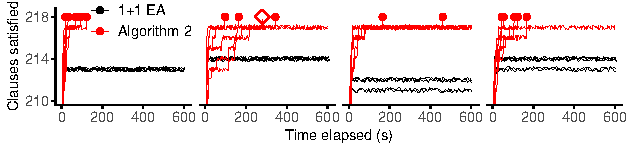
\includegraphics{figures/constraints-over-time.pdf}}} \\
    \raisebox{-\height}{B} & %
    \raisebox{-\height}{\includegraphics{figures/populationsize-over-time.pdf}} & %
      \raisebox{-\height}{C} & %
      \raisebox{-\height}{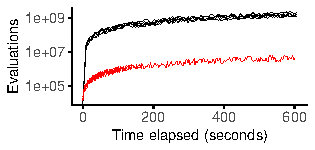
\includegraphics{figures/evaluations-over-time.pdf}}
  \end{tabular}
  \endgroup
  \caption{
    Algorithm~\ref{algorithmweightedea}'s population expands out of local optima.
    (A)
    Algorithm~\ref{algorithmweightedea} ($r=3$, $p=0.99$) and a
    1+1-EA ($p_m = 0.02$) running on four Boolean satisfiability problems.
    Jitter is added in the y direction and the y-axis is interrupted
    at 210 clauses.
    The diamond in the top right indicates a run for which in
    (B)
    population size is shown.
    Vertical dotted lines indicate when more clauses are satisfied.
    (C)
    Cumulative number of fitness evaluations for runs in the rightmost subplot of (A),
    counting two evaluations of the same string twice.
    Jitter is added in the y direction.
  }
   \label{satsolving}
\end{figure}

We investigated a collection of difficult satisfiability problems
from SATLIB called ``Uniform Random-3-SAT'' \cite{Hoos2000}.
This collection consists of randomly generated
problems with a fixed number of clauses and variables 
that are unusually difficult to solve \cite{Cheeseman1991,mitchell1992}.
We expected such problems to have a glassy solution landscape
\cite{Kirkpatrick1994}, and hypothesized that an EA operating in 
such a landscape might benefit from Algorithm~\ref{algorithmweightedea}'s
ability to support large population sizes.

We selected four satisfiable problems with 50 variables and 218 clauses
at random from the ``Uniform Random-3-SAT'' collection to run our EAs on.
We performed six runs of both EAs on each problem,
cutting them short if no solution is found in ten minutes.
Algorithm~\ref{algorithmweightedea} and the 1+1-EA both find strings
that solve at least 210 of the clauses within seconds
(Figure~\ref{satsolving}A).
In all runs, our
1+1-EA got stuck in a local optimum after these first seconds.
Algorithm~\ref{algorithmweightedea} finds new optima comparatively
quickly.
When Algorithm~\ref{algorithmweightedea} finds a new optimum,
its population size falls (Figure~\ref{satsolving}B),
because the pruning step removes strings that solve too few
clause with respect to the newly found best string.
During a stall, the population grows,
building up an increasingly large repository of high fitness strings
from which to expand further.

A single ``clutch'' of offspring consists of 20876 strings,
whose fitness is evaluated concurrently in $n+1$ automata operations.
However, this large amount of simultaneous fitness evaluations alone does not 
explain why Algorithm~\ref{algorithmweightedea} find the optimum faster;
in fact, the 1+1-EA performs two orders of magnitude more fitness evaluations
per time unit (Figure~\ref{satsolving}C).
%
Taken together, a picture emerges of how
Algorithm~\ref{algorithmweightedea} escapes local optima.
Each round, a clutch of 20876 strings is inserted into a population
whose size never exceeds 20000.
Almost all offspring does not survive their first iteration.
Stringent selection notwithstanding,
the population keeps expanding into new territory,
keeping above a ``waterline'' set by pruning.
When encountering higher territory,
this ``waterline'' is raised accordingly.

\label{sectionwaga}
\section{Discussion and Future Work}

In this paper, we have developed and tested an approach to implement
population compression for population-based algorithms that use
weighted strings. Our approach is an extension of earlier work in the
AIS field \cite{Liskiewicz2010} that supports weighted instead of
unweighted populations. We have demonstrated that (1) the addition of
weights can considerably improve the performance and robustness of AIS
algorithms; (2) the addition of weights makes it possible to leverage
the population compression approach for implementing an EA. 
We are not aware of other EAs based on (W)FSMs, although 
there are other approaches to represent populations
in compressed or implicit form \cite{Baluja1995,Harik1999,Manso2009}.
In contrast to these approaches, FSMs allow for mass operations performed on
all strings simultaneously. 
%% For example, in the proposed algorithm we take a mutational
%% neighborhood, evaluate all strings within it, and prune the worst ones
%% in just a handful of FSM operations.
%\textbf{Need a concluding sentence.}
%% Simple operations on an FSM can modify a large number of strings,
%% enabling operations otherwise unfeasible in a GA.

%% an impressive body of work considers how we may best represent the
%% (candidate) solutions \cite{Ronald1997,Rothlauf2006},
%% there is literature where these entities themselves are finite state
%% machines (e.g. \cite{Fogel1995,Alvarez2011,Masek2018}),

%% 1. Our pruning corresponds biologically to fierce competition for
%%    an essential resource.  Such a competition regime may facilitate
%%    what evolutionary biologists may call pulsed evolution
%%    \cite{Pennel2014} or punctuated equilibria \cite[Chapter
%%    20]{Futuyma2017} by introducing repeated bottlenecks.  This
%%    would funnel the population into local optima, decreasing
%%    diversity along the way.  This funneling tendency is apparently
%%    counteracted by aggressive exploration.

%% 2. Although larger clutch sizes lead to superlinear speedup, number
%%    of evalutations over time are smaller for Algorithm 2 than for
%%    1+1 EA.  Suggests that ours is a good search strategy, but not
%%    necessarily a good implementation for it (On the Utility of
%%    Populations in EAs)

%% 3. Adding the whole mutational neighborhood for offspring is novel
%%    as far as I'm aware.  Close analogy is supermutation operator in
%%    AISs (where they may help breaking out of local minima -- ppsn
%%    AIS paper)

%% 4. Apparent plateaus in solution space at higher connectivity.

%% 5. Use of FSAs!
It is important to mention some limitations of our approach. Compared to more standard implementations of a population-based algorithm, using WFSMs requires significantly more advanced algorithms and data structures. To some extent, this is mitigated by the availability of WFSM libraries, but some issues remain. First, building WFSM-based population algorithms may require
merging very large numbers of small classifiers. The OpenFST framework we currently use
implements WFSM union in a way that does not yield a minimal result, such that we need
to call minimization after every union to keep FSM size manageable. % for example, it aggressively 
%re-distributes WFSM edge weights. In theory, this keeps the weights in a normalized state 
%such that minimization keeps the WFSM at minimal size. Yet this comes at a cost of 
%potential loss of precision that is not important when performing only a few operations, 
%but can rapidly compound to massive issue when many operations are performed 
%(Figure~\ref{figurefpvsrationals}). 
Second, handling weights in WFSMs proved to be more challenging than we
anticipated. Our use of exact rational algebra proved critical to get our WFSM-AISs 
to work even on small  input samples -- without it, even populations trained on as 
few as 1000 input characters could rapidly blow up to 100s of megabytes in size. 
While the use of rationals greatly improved this and allowed us to perform the
experiments reported in this paper, it is not a complete solution because the rationals
themselves could eventually ``blow up'' and use numerators or denominators that are too 
large to be represented as integers. 
%In such  cases quantization becomes necessary, bringing back the issue that strings with 
%equal weights may no longer be recognized as such. 
While this did not cause any major 
issues in the experiments reported in this paper, we expect it to become problematic 
when storing large numbers of strings with very different weights at very different 
orders of magnitude. 

On the other hand, these new issues that we encountered while using WFSMs in a new 
application domain might lead to interesting research questions: how can we develop
fast and robust algorithms for use with very large numbers of small FSMs and related
operations on them? For unweighted FSMs with a ``levelled'' structure that population
models typically use
(i.e., acyclic FSMs where all paths between two nodes have the same length),
Textor \emph{et al.} \cite{Textor2014} implemented a custom FSM union algorithm that directly 
outputs a minimal FSM. This could be extended to WFSMs in future work. 
Likewise, we could use a directly 
determinizing union algorithm like the one by Mohri \cite{Mohri1996}, created for a 
similar use-case. Minimization may also be sped up by the algorithm of 
Eisner \cite{Eisner2003}. Since WFSMs are 
generic data structures that are used in many different fields, such research may be 
useful outside of the context of natural computing. We look forward to working on 
such issues with researchers in the automata community. 


We expect our approach to be applicable to many population-based algorithms. The most obvious candidate is perhaps the learning classifier system (LCS) \cite{Urbanowicz2009}. Surprisingly, the close similarity of AIS and LCS has not been explored much in the literature -- even though the original motivation behind these algorithms is very different, a LCS can in fact be viewed as a more sophisticated version of an AIS where positive or negative selection is only an initial step to build the classifier population, which is then evolved further by reinforcement learning. We hypothesize that the WFSM framework developed in this paper should be equally useful to increase the scale of LCS such that richer, more interesting problems can be studied. We hope that the insights gleaned from such work will allow us to better understand 
parallel distributed information processing systems in Nature, including but not limited to the immune 
system.


\begin{credits}
  \subsubsection*{\ackname}
  JT and GS were supported by NWO grant VI.Vidi.192.084 (to JT).
  \subsubsection*{\discintname}
  The authors do not declare any conflict of interest.
\end{credits}

\bibliography{references}

\end{document}




%%% OLD PARTS THAT ARE NO LONGER USED


\section{Conclusion}

AIS were originally invented in the 1990s, a time in which modern ML/AI technology did not 
yet exist, and anomaly detection problems -- especially sequence-based ones -- were hard to 
solve. Nowadays with sequence-based end-to-end learning and transformers, anomaly detection
in sequence data can be approached using state-of-the-art neural network models. Such models
can scale to millions or billions of parameters to learn semantic features of large sequence datasets.
Despite our  contributions in this paper, AIS models are not yet optimized anywhere nearly as well. Crucially, 
such approaches are gradient-based, whereas AIS remains essentially a grandient-free approach.
Even before all this, Stibor wrote already in 2006 that 
(negative selection) ``was thoroughly explored'' and that ``future work in this direction is not meaningful''
\cite{Stibor2006}. Why, then, still bother with AIS? 

We do agree that AIS is unlikely to become a competitive technology for anomaly detection 
in sequence data anytime soon. We disagree, however, that AIS has been ``thoroughly explored''.
For example, our simple experiments with noisy classification problems in Section~\ref{sectionempirical}
have revealed a new fundamental issue with the decades-old negative selection algorithm
\footnote{Technically, we showed these results for positive selection, but the results for
negative selection would be the same (Remark~\ref{remarkbotharethesame}).}: its performance degrades when the input data becomes too large.
This fundamental issue has (to our knowledge) 
never been pointed out before, possibly because without FSM-based AISs, it has not 
been possible to build systems of the scale required to even allow processing of inputs of this size. 
This shows how we need to build such systems at scale to fully understand their properties.

Currently, the most important motivation to carry out this work
is to study the information processing capacity of the immune system itself, which remains
incompletely understood. For example, recent data cast substantial doubt on 
the long-standing immunological theory of negative selection, which the eponymous algorithm
is based on. Repertoire models have been instrumental to place these new findings into context
and to develop a more fine-grained understanding of the function of selection processes in
 the thymus. Again, such models need to be large-scale to be useful, because real immune
systems contain many millions to billions of cells.

Beyond computational immunology, we are intrigued by the fact that the close similarity of AIS
repertoire models and learning classifier systems (LCS) has not been explored further. LCS 
have similar issues as AIS around scale and (doubts about) usefulness, although LCS are typically
used in a reinforcement learning setting where the ability to process very large sets of input
data is not immediately critical. While the AISs we considered in this paper focused mostly 
on the initial stages of repertoire development -- positive and negative selection -- the processes
occurring throughout an individual's lifetime are more akin to reinforcement learning: pathogens
are recognized, eliminated and memorized through an evolution-like process, which in the case
of B~cells also involves mutation of the repertoire sequence and fitness-based selection
(affinity maturation). Therefore, we feel that (repertoire-based) AISs should ultimately 
be seen as a special case of LCS. We hypothesize that the WFSM framework developed in this paper 
should be equally useable to increase the scale of LCS such that richer, more interesting problems
can be studied. We hope that the insights gleaned from such work will allow us to better understand 
parallel distributed information processing systems in Nature, including but not limited to the immune 
system.






%\subsection{Motivation and prior work}
% Diversity 
Artificial neural networks that underlie the rapid advances in AI/ML in recent years, 
from convolutional neural networks to transformers, 
were originally inspired by computational models of the human brain. Intriguingly, our bodies contain a 
second complex adaptive information-processing system that learns through an entirely
different mechanism: the immune system. Unlike the brain, which derives its complexity 
from connections between cells of the same type, the immune system's pattern 
recognition cells -- B and T~cells -- are much more diverse, mainly due to specific 
genetic machinery that randomly generates parts of their DNA sequence. For example, 
the number of different T~cells that can be made due to this mechanism is estimated 
to be in the range of $10^{15}$ to $10^{20}$ \cite{Zarnitsyna2013}, many orders of 
magnitude more than the number of bits stored in the human genome. Each of us harbors
 only around $10^{11}$ T~cells, a small fraction of what can be realized, meaning that many of our T~cells are fairly unique in the population. This large and diverse amount of cells is very expensive to make (the entire process takes until adulthood in humans) and to maintain. Why is such a large number of cells necessary?

%Specificity 
Each adaptive immune cell specializes on recognizing very specific molecular patterns 
called \emph{epitopes}. For T~cells, the epitopes are short amino acid sequences (peptides) 
that originate as waste products from every cell's protein degradation machinery. 
Specifically, the CD8$^+$ subpopulation of T~cells recognizes epitopes about 9 amino acids 
long, and the CD4$^+$ subpopulation recognizes longer peptides in the range of 12-14 
amino acids. For any given peptide, the fraction of T~cells in the immune system that will 
recognize it is thought to be on the order of 10$^{-5}$ \cite{Blattman2002}. 
Since immune cells need to protect us from a vast amount of pathogens, some of which may not 
 even exist yet, they need to completely cover the space of possible antigens. 
 This is why so many cells need to be made and maintained. 
 \footnote{This energy expense is even more costly for smaller animals such as mice. 
 A mouse consists of ~$3\times 10^9$ cells and  ~$10^8$ of these -- or 5-10\% of the 
 entire animal -- are adaptive immune cells.}

% Negative selection algorithms
Computer scientists have long been interested in the computational properties and 
capacities of the immune system, and particularly of its adaptive arm, starting with 
pioneering work by Stephanie Forrest, Alan Perelson, and others in the 
1990s \cite{Forrest1990,Percus1993}. Algorithmic models of the immune system -- 
now called \emph{artificial immune systems} (AIS) -- are often built around the notion 
of large \emph{repertoires} (sets) of small, specific classifiers called \emph{detectors} 
or \emph{patterns}, a property shared with more generic \emph{learning classifier systems} 
(LCS) \cite{Wilson1994}. One of the earliest AISs, Forrest's negative selection algorithm \cite{Forrest1994}, 
was based on the ``education'' of T~cells during negative selection in the thymus: 
upon randomized rearrangement of their receptor sequence, T~cells get shown ``normal'' 
peptides from the host's cells, and those that respond to one of these normal ``self'' 
peptides are killed. This simple process was thought to ensure that T~cells react only 
to the ``nonself'' peptides that would arise, for example, when cells get infected by a 
virus or mutate and become cancerous. More recent data has now cast some doubt on this 
However, the negative selection algorithm still works in principle, and AISs have also 
been used in computational immunology to revisit the negative selection theory in light 
of the new data \cite{Wortel2020t}.

% Importance of scale
After initial enthusiasm led to the establishment of a research community around 
AIS, it quickly became clear that scale was a central issue in such systems. Like in the 
real immune system, AISs had to provide very large numbers of classifiers to cover the 
entire possible problem space, and the number of classifiers required  often scaled 
exponentially with important parameters of the system. The inability to build AISs at the 
 scale required to solve challenging real-world problems may have been partly 
 responsible for the decline of the AIS field in the 2000s. However, algorithmic models 
 of the immune system continue to be relevant in (computational) immunology itself, 
where they are used to improve our understanding of adaptive immune responses, and  
ultimately to predict such responses. Again, the use of AISs in computational immunology 
requires systems that are large enough to ask and address relevant questions. 

It is perhaps instructive to compare AIS to artificial neural networks, 
which went through an extended period of relative obscurity. Incremental 
improvements in scale and efficiency were made -- until it suddenly became clear 
that all these ``incremental'' developments taken together massively improved the utility 
of such systems. Equally, we feel that AIS models deserve the attention to 
detail needed to build them efficiently and at scale, in order to really 
understand how these systems work and what they are capable of.

% FSTs
An important development in AIS methodology has been the idea that 
\emph{compressed representations} of detector repertoires can be used to build much 
more efficients AISs. This idea was initially used to debunk claims \cite{Timmis2008} 
that detector generation for negative selection with so-called  
r-chunk and r-contiguous detectors is an NP-hard problem \cite{Elberfeld2011}. It was 
later shown how \emph{finite state machines (FSMs)} can be used as a generic building 
block to build such compressed representations for arbitrary string matching rules, 
although for some matching rules such compressed representations will still have an 
exponential size in the worst cases \cite{Liskiewicz2010}. 
Recently, an FSM-based AIS was used to build an algorithmic model of negative selection 
consisting of tens of millions of detectors that processed the entire human proteome 
as input \cite{Wortel2020t}. 

However, these FSM-based AISs still have important limitations. Crucially, they represent 
detector repertoires as sets without multiplicity. This means that all detectors in the 
set will have equal importance or strength, which limits the complexity of the 
information that can be stored.

%\subsection{Our contributions}

In this paper, we present a new type of AIS repertoire models where each detector in a 
repertoire is assigned a weight, similar to how classifiers in LCS can be weighted. 
Specifically, we: 

\begin{enumerate}
\item Define weighted versions of positive and negative selection, two of the most important AIS algorithms  (Section~\ref{sectionbackground});
\item Show how weighted positive and negative selection can be implemented efficiently by using compressed repertoire representations based on weighted FSMs (Section~\ref{sectionfsms});
\item Illustrate the potential benefit of using weights by comparing the performance of weighted versus unweighted repertoire models on simple string-based anomaly detection problems (Section~\ref{sectionempirical}).
\end{enumerate}

